%%%%%%%%%%%%%%%%%%%%%%%%%%%%%%%%%%%%%%%%%%%%%%%%%%%%%%%%%%%%%%%%
% Sablona pro zaverecnou zpravu k semestralni praci z BI-ZUM
% Kódování dokumentu: UTF8
% Verze: 1.0 (2013-01-28)
% Autor: Ing. Martin Šlapák
%%%%%%%%%%%%%%%%%%%%%%%%%%%%%%%%%%%%%%%%%%%%%%%%%%%%%%%%%%%%%%%%
%
% NEUPRAVUJTE PROSIM PARAMETRY DOKUMENTU, JAKO OKRAJE CI PISMO!
%
%%%%%%%%%%%%%%%%%%%%%%%%%%%%%%%%%%%%%%%%%%%%%%%%%%%%%%%%%%%%%%%%
%
% Celkova delka zpravy nesmi presahnout 1 stranu A4, vyjadrujte 
% se strucne, jasne a vecne - zadne omacky a slovni vata. Diky!
% Neprehazujte ani poradi sekci.
%
%%%%%%%%%%%%%%%%%%%%%%%%%%%%%%%%%%%%%%%%%%%%%%%%%%%%%%%%%%%%%%%%
\documentclass[a4paper,10pt,twocolumn]{article}
\usepackage{lmodern}
\usepackage[czech]{babel}
\usepackage[T1]{fontenc}
\usepackage[utf8]{inputenc}
\usepackage{graphicx}
\usepackage{float}
\usepackage[top=0.5cm,bottom=2cm,left=1cm,right=1cm]{geometry}
%gobble sezere cisla stranek, takze nebudou zadna
\pagenumbering{gobble} 
\title{Zpráva k 3. domácímu úkolu z předmětu MI-PAA}
\date{\today}
%%%%%%%%%%%%%%%%%%%%%%%%%%%%%%%%%%%%%%%%%%%%%%%%%%%%%%%%%%%%%%%%
% tady nastavte své jméno a email
\author{Jan Sokol \\ sokolja2@fit.cvut.cz}
%%%%%%%%%%%%%%%%%%%%%%%%%%%%%%%%%%%%%%%%%%%%%%%%%%%%%%%%%%%%%%%%
\begin{document}
\maketitle
%%%%%%%%%%%%%%%%%%%%%%%%%%%%%%%%%%%%%%%%%%%%%%%%%%%%%%%%%%%%%%%%
\begin{abstract}
% Úkolem bylo nalézt řešení 0/1 problému batohu hrubou silou (tj. nalezení skutečného optima). Dále bylo třeba zkušebních datech pozorovat závislost výpočetního času na n (kde n je počet věcí v batohu). Druhou částí ukolu naprogramování řešení problému batohu dalšími, pokročilými metodami.
%  \begin{itemize}
% \item První byla metoda větví a hranic (B\&B). A to tak, aby omezujícím faktorem byla hodnota optimalizačního kritéria. Tj. při ořezávání shora omezení bylo překročení kapacity batohu. Omezení zdola bylo řešeno podmínkou, že stávající řešení nemůže být lepší než nejlepší dosud nalezené. Tato metoda je lepší (rychlejší) prořezávání prostorem, než je hrubá síla,
% \item metodou dynamického programování,
% \item FPTAS algoritmem, (tj. s použitím modifikovaného dynamického programování s dekompozicí podle ceny).

% \end{itemize} 
% Na těchto datech bylo třeba pozorovat závislost výpočetního času na n (a to také s metodami z minulé úlohy - hrubou silou a jednoduchou heuristikou).

Zadáním třetí úlohy bylo rozloženo do třech bodů. Tím prvním bylo prozkoumání citlivosti metod řešení problému batohu na parametry instancí generovaných generátorem náhodných instancí (přiloženým v zadání úlohy). V případě podezření na další závislosti nám bylo doporučeno, abychom modifikovali zdrojový tvar generátoru.
Na základě zjištění z minulého bodu jsme měli provést experimentální vyhodnocení kvality řešení a výpočetní náročnosti. 
Zkoumat jsme měli obzvlášt metody:
 \begin{itemize}
\item hrubá síla (pokud z implementace není evidentní úplná necitlivost na vlastnosti instancí),
\item metoda větví a hranic,
\item dynamické programování (dekompozice podle ceny a/nebo hmotnosti),
\item heuristika - poměr cena/váha.
\end{itemize} 

Na těchto metodách jsme měli zkoumat zejména závislost výpočetního času (případně počtu testovaných stavů) a rel. chyby (v případě heuristiky) na:
 \begin{itemize}
\item maximální váze věcí,
\item maximální ceně věcí,
\item poměru kapacity batohu k sumární váze,
\item granularitě.
\end{itemize} 


% Zde shrňte v několika větách co jste dělali, jak jste to dělali, jakých výsledků jste dosáhli. Vypíchněte to nejzajímavější. Zkusili jste nějakou pokročilou techniku? Tady se s ní pochlubte a pak ji dále rozepište v patřičné sekci. Zkuste se vejít do 150 slov.
\end{abstract}

%%%%%%%%%%%%%%%%%%%%%%%%%%%%%%%%%%%%%%%%%%%%%%%%%%%%%%%%%%%%%%%%
\section{Výběr jazyka}
Pro svou implementaci problému batohu jsem si vybral jazyk Python. Ačkoli to je jazyk interpretovaný a nečekal jsem závratné rychlosti výpočtů, mojím výběrem byl pro to, že jsem jazyk znal a pro jakýkolik koncept je pro mne nejrychlejší.

% V případě hledání řešení hroubou silou jsem těžil z materiálů v přednáškách, tak i na internetu.

% Metoda branch and bound zajišťuje, že prostor je prořezáván jak zdola, tak shora. Ty větve v rekurzi, které by neposkytly lepší výsledek (či by přesáhny kapacitu batohu), nejsou dále procházeny. V paměti držen nejlepší výsledek (globální hodnota). Před každým sestoupením do spodní větve se zkontroluje cena zbývajíchích (ještě nepřidaných) předmětů. Pokud součet cen zbývajících itemů a držené ceny batohu je menší, než nejlepší výsledek, k lepší hodnotě už se není možné dostat a průchod ukončujeme.

% Pomocí metody dynamického programování přesouváme náročnost na CPU na paměťovou náročnost. Vybral jsem dekompozici dle ceny - abych funkce dále mohl využít i pro metodu FPTAS. V paměti držíme tabulku (decomposition table), kam ukládáme mezivýpočty. Sloupce jsou ceny, řádky jsou předměty. Těmito mezivýpočty jsou aktuální váhy v batohu. Výsledek je poté možné vidět ve spodním řádku - ta hodnota, co je nejvíce napravo.

% Při výpočtu FPTAS můžeme ovlivnit kvalitu výsledku tím, že nastavíme proměnnou accurancy. Tou je možné definovat maximální relativní chybu, se kterou algoritmus bude pracovat. Zde jde o zanedbání určitého počtu bitů z ceny. Ceny předmětů jsou zpoměrovány, a poté je výpočet stejný, jako u dynamického programování.


\section{Testovací Hardware}
Všechny testy byly prováděny na cloudové linuxové instanci v AWS, běžící na Red Hat Enterprise Linux 7. Velikost instance byla:
  2 Core CPU / 8 GB RAM, v názvosloví AWS \textbf{m4.large}.


\section{Měření výpočetního času}
Výpočet běhu funkce je řešen tak, že je spočten strojový čas před během funkce, a také po něm. Tyto časy jsou od sebe odečteny a je vrácen čas v ms.

   \begin{verbatim}
def timing(f):
    def wrap(*args):
        time1 = time.time()
        ret = f(*args)
        time2 = time.time()
        measured_time.append(
          {'type': f.__name__,
           'time': (time2-time1)*1000.0})
        return ret
    return wrap
   \end{verbatim}


\subsection{Postup experimentu a vybrané parametry}

Jako vstup mého experimentu jsem zvolil závislost zkoumaného parametru z abstraktu (maximální váha věcí, maximální cena věcí,
poměr kapacity batohu k sumární váze a granularita) na dvou mnou vybraných parametrech - času běhu řešení instance daným algoritmem dosažení spočtené ceny. Pro zjednodušení celého experimentu jsem postup vždy udělal stejný, jen se změněnými parametry.

Oba typy experimenty měly stejně definovány jejich výstupy. Jak u jednoho, tak i u druhého jsme schopni popsat kvalitu algoritmů, jen lehce jiným způsobem. 

Závislost vypočtené průměrné ceny na definovaném parametru ze zadání může být občas nepřesné a zavádějící. Například v experimentu, kde měníme maximální cenu věcí, s parametry:
   \begin{verbatim}

'items': 10, 'instances': 10, 
'capacityratio': 0.5, 'maxweight': 100,
 'maxprice': 10, 'exp': 4, 'balance': 0
    \end{verbatim}

\begin{figure}[H]
  \begin{center}
    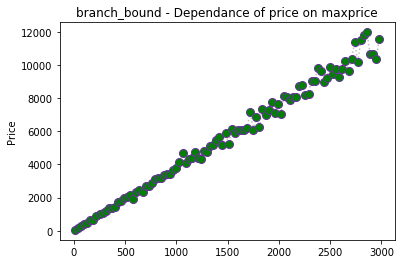
\includegraphics[height=6cm]{graphs/price_on_maxprice_branch_bound.png}
  \end{center}
  % \caption{Graf vývoje fitness}\label{fig1}
\end{figure}

Když je experiment nastaven tak, že je dostupných jenom 10 předmětů (s jiejich maximální hodnotou 1), tak se nemůže stát, že by celková hodnota batohu přesáhla 10. A to vidíme přesně na grafu výše.

% \subsection{Výpočetní časy jednotlivých metod}


% \begin{figure}[H]
%   \begin{center}
%     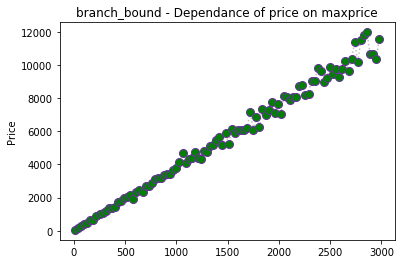
\includegraphics[height=6cm]{graphs/price_on_maxprice_branch_bound.png}
%   \end{center}
%   % \caption{Graf vývoje fitness}\label{fig1}
% \end{figure}



\section{Zkoumání maximální hodnoty věcí}


Při nastavení maximální ceny věcí na různé hodnoty, můžeme vidět že dynamickému algoritmu roste výpočetní čas se zvětšením maximální hodnoty.
   \begin{verbatim}

'algorithm': 'dynamic', 'id_inst': 0, 'items': 10,
'instances': 10, 'capacityratio': 0.5,
'maxweight': 100, 'maxprice': 10,
'exp': 4, 'balance': 0
\end{verbatim}

\begin{figure}[H]
  \begin{center}
    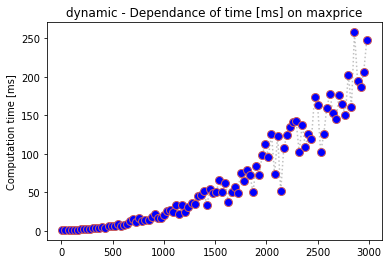
\includegraphics[height=6cm]{graphs/time_on_maxprice_dynamic.png}
  \end{center}
  % \caption{Graf vývoje fitness}\label{fig1}
\end{figure}

Časová závislost u dynamického programování v závislosti na maximální cenu věcí se zdá skoro exponenciální.

U všech ostatních metod je možné vidět, že maximální cena věcí výpočetní čas nijak neovlivňuje.
\section{Zkoumání maximální váhy věcí}

Algoritmus s heuristikou poměru cena/váha nám  na časovém grafu ukazuje mírně stoupající trend -- ale ten je nejspíše způsobem režií algoritmu (např. práce s pamětí, atp.).
Parametry:
   \begin{verbatim}

'algorithm': 'heuristic', 'id_inst': 0, 'items': 10,
'instances': 50, 'capacityratio': 0.5,
'maxweight': 15, 'maxprice': 25, 'exp': 4,
'balance': 0
    \end{verbatim}

\begin{figure}[H]
  \begin{center}
    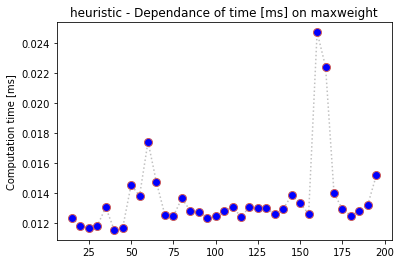
\includegraphics[height=6cm]{graphs/time_on_maxweight_heuristic.png}
  \end{center}
  % \caption{Graf vývoje fitness}\label{fig1}
\end{figure}


V cenových grafech jsem žádné závislosti či trendy nezaznamenal. Výsledky vypadají z většiny náhodně. Zde přikládám relevantní graf pro metodu heuristikou (se stejnými parametry jako výše), ostatní metody je možné vidět v přiloženém python notebooku. 

\begin{figure}[H]
  \begin{center}
    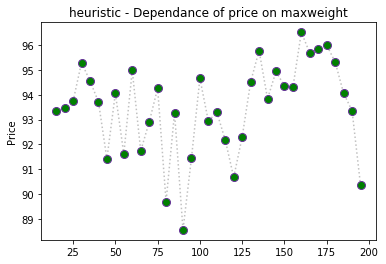
\includegraphics[height=6cm]{graphs/price_on_maxweight_heuristic.png}
  \end{center}
  % \caption{Graf vývoje fitness}\label{fig1}
\end{figure}

% graphs/time_on_maxprice_dynamic.png

\section{Zkoumání poměru kapacity k sumární váze}


Zajímavou reakci ukázal algoritmus Dynamické programování. Z grafu níže můžeme vypozorovat, že dynamické programování bylo efektivnější při menší kapacitě vůči sumární váze.

   \begin{verbatim}

'algorithm': 'dynamic', 'id_inst': 0, 'items': 10,
'instances': 5, 'capacityratio': 0.05,
'maxweight': 100, 'maxprice': 100, 
'exp': 4, 'balance': 0
                                   \end{verbatim}

\begin{figure}[H]
  \begin{center}
    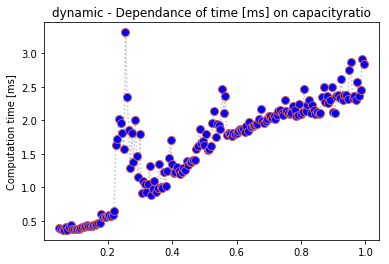
\includegraphics[height=6cm]{graphs/time_on_capacityratio_dynamic.png}
  \end{center}
  % \caption{Graf vývoje fitness}\label{fig1}
\end{figure}

Zatímco jak můžeme vypozorovat u algoritmu Branch and Bound, ta je nejvíce efektivní jak pro malé kapacity v poměru k sumární váze, tak i ty velké. (Pro poměr 50\% - 50\% byl algoritmus nejméně efektivní).

   \begin{verbatim}

'algorithm': 'branch_bound', 'id_inst': 0, 'items': 10,
'instances': 5, 'capacityratio': 0.05,
'maxweight': 100, 'maxprice': 100, 
'exp': 4, 'balance': 0
                                   \end{verbatim}

\begin{figure}[H]
  \begin{center}
    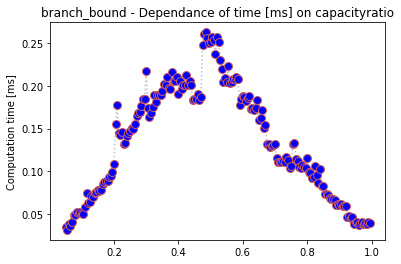
\includegraphics[height=6cm]{graphs/time_on_capacityratio_branch_bound.png}
  \end{center}
  % \caption{Graf vývoje fitness}\label{fig1}
\end{figure}


U ostatních metod jsem žádnou závislost poměru kapacity k sumární váze nevypozoroval. Rád bych znovu odkázal na Jupyter notebook, kde je toto možné vidět.

\section{Zkoumání granularity instancí}

Při zkoumání reakce algoritmů na změnu granularity jsem měnil exponent (proměnná exp v konfiguraci) v krocích po 0.005, od 0 do 1. Dále jsem měnil balanci mezi malými věcmi (parametr -k), který byl nastaven na -1, 0 a 1.

Nicméně při žádných změnách jsem na žádné závislosti nenarazil. Pro zobrazení měřených výsledků doporučuji nahlédnout do Jupyter notebooku přiloženém v repu.


\section{Shrnutí a výsledky}


Výsledky z experimentů v této úloze nám převážně potvrzují vědomosti nabyté v předchozích úkolech. 

Nejvíce mě překvapilo změnění poměru kapacity k sumární váze u metod branch and bound a dynamického programování. Z výsledků jsou mi jasné jednotlivé výhody a nevýhody algoritmů při změněných parametrech.

Dále bylo zajímavé pozorovat změnu maximální hodnoty věcí u dynamického programování, kdy výpočetní složitost algoritmu rostla velmi rychle při zvětšování proměnné.

Pro vytváření grafů bylo využito Python notebooku, který je přiložen v adresáři \textbf{report/report3/experiments.ipynb}, případně z něj vygenerovaný markdown soubor v \textbf{report/report3/data/experiments.zip}. Grafy jsou vykresleny pomocí knihovny \textbf{mathplotlib}.

Data vypočtená z generátoru a běhu algoritmu je možné vidět v tomto repozitáři, v cestě \textbf{report/report3/}. Tento adresář také obsahuje funkce, pomocí kterých bylo experimentu dosaženo a pomocí kterých byly grafy vygenerovány.

% Tady okomentujte k čemu se váš evoluční algoritmus dopracoval, co se vám povedlo, co ne a jak by to šlo vylepšit. Jakého nejlepšího řešení se vám podařilo dosáhnout. Klidně i napište, co se vám na semestrální práci líbilo a taky co byste raději měli jinak. Uvítáme jakékoli nápady. 

% Pokud jste čerpali z nějaké literatury, měli byste ji řádně ocitovat.

% \textbf{A NEZAPOMEŇTE, ŽE SE MUSÍTE VEJÍT NA JEDNU A4! ;-)}

%%%%%%%%%%%%%%%%%%%%%%%%%%%%%%%%%%%%%%%%%%%%%%%%%%%%%%%%%%%%%%%%
% odtud dal to pak zakomentujte pomoci znaku procenta na zacatku radku
% \begin{center}
% \line(1,0){250}
% \end{center}

% \textbf{Pár poznámek pod čarou\ldots}
% \begin{itemize}
%   \item Zdroják této šablony je v kódování UTF8.
%   \item Neměňte prosím žádná nastavení dokumentu, okrajů, velikosti písma apod.
%   \item Nepřehazujte ani pořadí sekcí.
%   \item \textbf{Jak zprávu zkompilovat?} Použijte dvakrát (kvůli odkazům a referencím) tento příkaz:

%   \begin{verbatim}
%   pdflatex zdrojak-zpravy.tex
%   \end{verbatim}

%   Výsledkem bude \textbf{zdrojak-zpravy.pdf}. 

%   \item Pokud něco nepůjde, konzultujte na cvičeních BI-TED či se spolužáky. Cvičící BI-ZUM nebudou mít čas řešit detaily s {\LaTeX}em.
%   \item \textbf{Proč se sakra musím vejít na 1 A4?} Chceme, abyste si vyzkoušeli jak napsat to podstatné, vybrat to důležité, vyhnout se takové té textové vatě. Současně po vás nechceme psaní dlouhých esejí, raději svůj čas věnujte svým algoritmům. A taky, kdo má číst 5 stran napsaných \uv{protože to chtěj}. ;-)
%   \item TIP: Tuto zprávu může být reálné uplatnit i jako jeden z domácích úkolů na BI-TED. K tomu vás ale nenutíme a také počítejte s tím, že tam po vás mohou chtít další rozšíření dokumentu. \textbf{Ale zase: proč nezabít dvě mouchy jednou ranou?}
% \end{itemize}

\end{document}
